\documentclass{DateStructure}

\SubjectName{教学计划编制问题}
\CollegeName{理学院}
\Major{信息与计算科学}
\GroupNumber{第十六组}
\StudentA{20071226}{童繁}{流程图}
\StudentB{20071227}{王瀚功}{数据}
\StudentC{20071228}{王赛豪}{文案}
\StudentD{20071229}{吴政豪}{调试}
\StudentE{20071230}{武琦}{代码}

\begin{document}
\makecover
\newpage
\thispagestyle{empty}
\tableofcontents   
\newpage
\setcounter{page}{1}  

\section{需求分析}
\begin{itemize}
\item[(1)]每个专业开设的课程都是确定的,而且课程在开设之间的安排必须满足先修关系。每门课程有哪些先修课程是确定的,可以有多门,也可以没有,每门课占一个学期。试在这样的前提下设计一个教学计划编制程序。
\item[(2)]输入参数包括:学期总数(不超过12),一学期的学分上限,每门课的课程号、学分和直接先修课的课程号,课程总数不超过100。如果输入的先修课程号不在该专业开设的课程序列中,则作为错误处理。
\item[(3)]允许用户指定下列两种编排策略之一:一是使学生在各学期中的学习负担尽量均匀;二是使课程尽可能地集中在前几个学期中。
\item[(4)]若根据给定的条件问题无解,则报告适当的信息;否则将教学计划输出到用户指定的文件中,并设计计划的表格格式。
\item[(6)]产生多种不同的方案,并使方案之间的差异尽可能地大。
\end{itemize}

\section{项目亮点}
如果有向图无回路,用户可以自行选择生成2-10种差异很大的拓扑排序序列;否则系统提示无法设计教学计划。
\section{概要设计}
拓扑排序是一个有向无环图的所有顶点的线性序列,每个有向无环图可以产生多种不同的序列。设计使用邻接表构建有向图,为产生差异较大的序列,这里将入度为0的顶点存入线性表,首先正序和逆序输出线性表,即为两种拓扑序列。然后利用线性表的特点和随机函数从表中随机输出顶点,即为更多的拓扑序列。

\section{详细设计}
\subsection{创建有向图}	
如果读取文件时同时读取课程编号和先决条件,当课程编号顶点未建立时,无法形成对应的弧,如C6的先决条件是C11,但此时未建立顶点C11,无法形成边。\par
因此首先读取用户指定的文件,第一行为学期总数、每学期最大学分上限、课程总数;第二行为所有课程编号,先建立顶点,再读取先决条件;之后的每一行为对应的学分和先决条件。在读取结束后,将生成对应的有向图。
\begin{lstlisting}[language=c,caption={Create}]
int Create(AlGraph* G)   //创建有向图
{
	int i,j,s,count;
	char a,name[30],str[4];
	FILE *fp;
	printf("<<<---教学计划编制系统--->>>\n");
	A:printf("请输入课程表文件名:");
	fflush(stdin);gets(name);strcat(name,".txt");
	if((fp=fopen(name, "r"))==NULL) {printf("该文件夹下无%s,请重新输入!\n",name);goto A;}
	G->message=(Term *)malloc(sizeof(Term));
	G->courses=(ClassNode *)malloc(sizeof(ClassNode)*G->vexNum);
	fscanf(fp,"%d%d%d\n\n",&G->message->termNum,&G->message->maxCredit,&G->vexNum);
	if(G->message->termNum>12||G->message->termNum<1||G->message->maxCredit<1
||G->vexNum>100||G->vexNum<1)
		{printf("输入超出范围!\n");return 0;}
	for(i=0;i<G->vexNum;i++)   //初始化
	{
		fscanf(fp,"%s",G->courses[i].classNum);
		G->courses[i].firstEdge=NULL;
		G->courses[i].inDegree=0;
	}
	for(i=0;i<G->vexNum;i++)
	{	
		fscanf(fp,"%d",&G->courses[i].credit);   //读取课程编号和学分
		while(fgetc(fp)!='\n')   //根据先决条件建立邻接表结点
		{
			fscanf(fp,"%s",str);
			s=(strlen(str)==2)?str[1]-'1':(str[1]-'0')*10+str[2]-'1';   //课程字符串转数字
			if(s<0||s>G->vexNum) {printf("%s输入错误!\n",G->courses[i].classNum);return 0;}
			EdgeNode *p=(EdgeNode*)malloc(sizeof(EdgeNode));   //更新邻接表结点
			p->adjVex=i;
			p->next=G->courses[s].firstEdge; 
			G->courses[s].firstEdge=p;
			G->arcNum++;
		}
	}
    fclose(fp);
	for(i=0;i<G->vexNum;i++)
	{
		for(EdgeNode *p=G->courses[i].firstEdge;p!=NULL;p=p->next) G->courses[p->adjVex].inDegree++;
	}
	return 1;
}
\end{lstlisting}
\subsection{拓扑排序}
利用有向图和线性表产生拓扑序列,将入度为0的点存入线性表,相关的邻接点入度减一,然后按照指定的规则从线性表中输出一个顶点,重复以上过程至线性表为空。\par
如果输出个数不为顶点个数,则说明有向图中存在环,提示用户无法生成拓扑序列。\par
用户自行指定使用其中一种序列作为教学计划顺序。
\begin{lstlisting}[language=c,caption={TopSort}]
int TopSort(ClassNode g[],int n,ClassNode *temp,int type)   //拓扑排序
{
	int i,j,k,m=0,gd[n],x;
	for(i=0;i<n;i++) gd[i]=g[i].inDegree;
	List degree;
    degree.length=0;
	EdgeNode* p;
	if(type==1||type>=a/2) for(i=n-1;i>=0;i--) {if(gd[i]==0) Add(&degree,i);}
	else for(i=0;i<n;i++) {if(gd[i]==0) Add(&degree,i);}
	printf("\n%d种拓扑排序结果为:",type);
	while(degree.length!=0)
	{
		if(type<3) x=0;
		else x=rand()%degree.length;
		j=degree.data[x];   //输出链表的某个元素
		Remove(&degree,x+1);
		printf("%s  ",g[j].classNum);
		temp[m++]=g[j];
		for(p=g[j].firstEdge;p;p=p->next)   //删除顶点j的所有出边
		{
			k=p->adjVex;
			if(!(--gd[k]))   //若顶点k入度为零则入链表
			{
				if(type==2) Insert(&degree,1,k);
				else if(type<a/2) Add(&degree,k); 
				else Insert(&degree,1,k);
			}
		}
	}
	if(m<n) {printf("AOV网有回路,无法设计教学计划!");return 0;}
	return 1;
}
\end{lstlisting}
\subsection{课程安排方案}
\subsubsection{均匀安排课程}
\begin{lstlisting}[language=c,caption={SortA}]
void SortA(ClassNode* t,Term* s,int classNum)   //均匀安排课程
{
    char name[30];
	printf("请输入教学计划编制文件名:");
	fflush(stdin);gets(name);strcat(name,".csv");
	FILE *fp=fopen(name,"w");
	printf("均匀安排课程的方案如下:");
	fprintf(fp,"学期,\t,课程");
	int i,j,b,c=0;   //用于输出课程信息
	for(i=0;i<s->termNum;i++)
	{
		b=0;   //累计每学期学分
		printf("\n第%d个学期的课程为:",i+1);
		fprintf(fp,"\n第%d学期,\t,",i+1);
		for(j=0;j<classNum/s->termNum;j++)
		{
			if(b+t[c].credit<=s->maxCredit)   //判断是否超过最大学分
			{
				if(c==classNum) break;
				printf("%s  ",t[c].classNum);
				fprintf(fp,"%s,",t[c].classNum);
				b=b+t[c].credit;   //学分累计
				c++;   //指向下一课程
			}
		}
		if(i<classNum%s->termNum)   //加入平均后多余的课程
		{
			if(c==classNum) break;
			printf("%s ",t[c].classNum);
			fprintf(fp,"%s,",t[c].classNum);
			b=b+t[c].credit;
			c++;
		}
	}
	fclose(fp);
}
\end{lstlisting}
\subsubsection{尽快安排课程}
\begin{lstlisting}[language=c,caption={SortB}]
void SortB(ClassNode* t,Term *s,int classNum)   //尽快安排课程
{
	char name[30];
	printf("请输入教学计划编制文件名:");
	fflush(stdin);gets(name);strcat(name,".csv");
	FILE *fp=fopen(name,"w");
	printf("尽快安排课程的方案如下:");
	fprintf(fp,"学期,\t,课程");
	int i,b,c=0;		
	for(i=0;i<s->termNum;i++)
	{
		b=0;   //累计每学期学分
		printf("\n第%d个学期的课程为:",i+1);
		fprintf(fp, "\n第%d学期,\t,",i+1);
		while(b+t[c].credit<=s->maxCredit)   //判断是否超过最大学分
		{
			if (c==classNum)break;
			printf("%s  ",t[c].classNum);		//输出课程
			fprintf(fp,"%s,",t[c].classNum);
			b=b+t[c].credit;   //学分累计
			c++;   //指向下一课程
		}
	}
	fclose(fp);
}
\end{lstlisting}

\section{用户手册}
\subsection{测试数据}
\lstinputlisting[language=C]{./测试/数据.txt}
\subsection{测试结果}
\begin{figure}[H] 
\centering
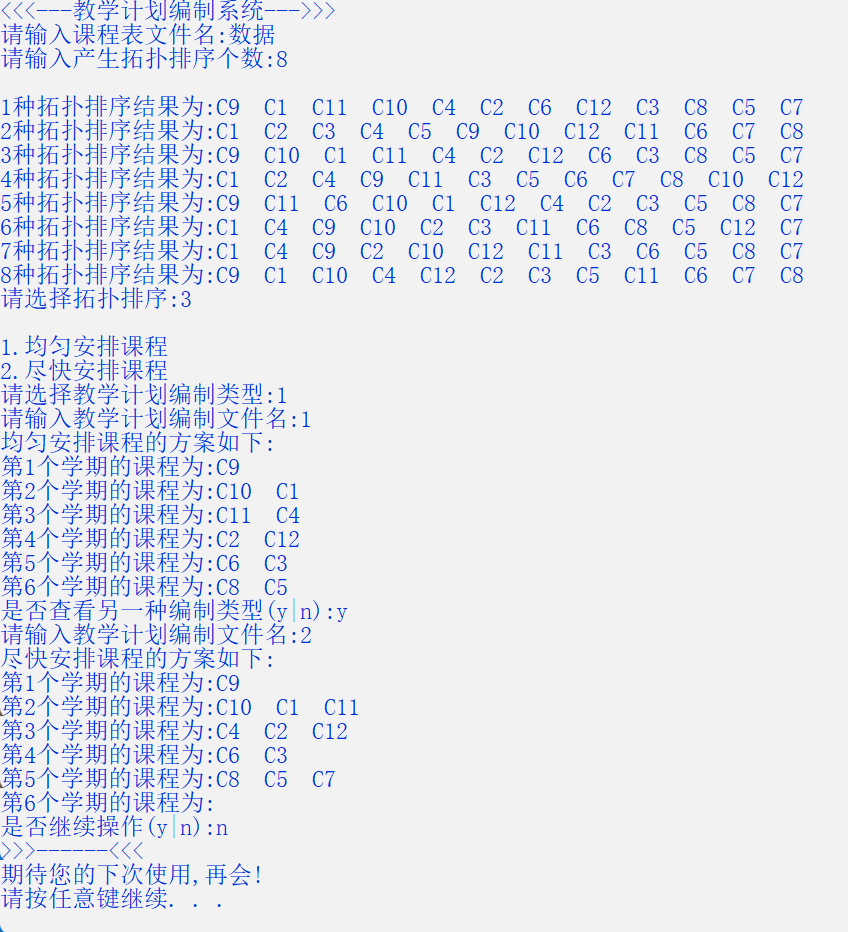
\includegraphics[width=300pt]{测试.png}
\caption{测试结果}
\end{figure}
\begin{figure}[H] 
\centering
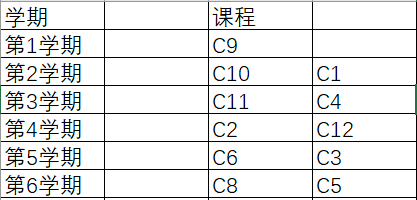
\includegraphics[width=300pt]{1.png}
\caption{均匀安排课程}
\end{figure}
\begin{figure}[H] 
\centering
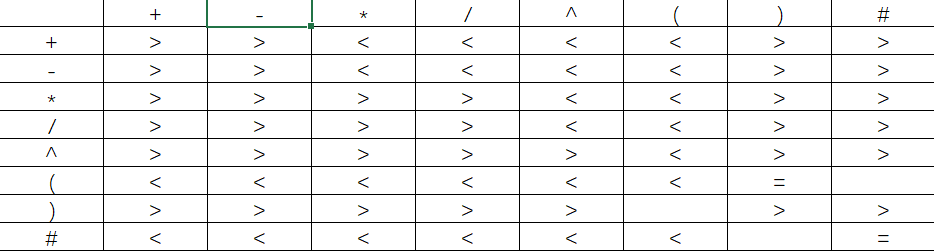
\includegraphics[width=300pt]{2.png}
\caption{尽快安排课程}
\end{figure}
\subsection{错误案例}
\lstinputlisting[language=C]{./测试/错误案例.txt}
\begin{figure}[H] 
\centering
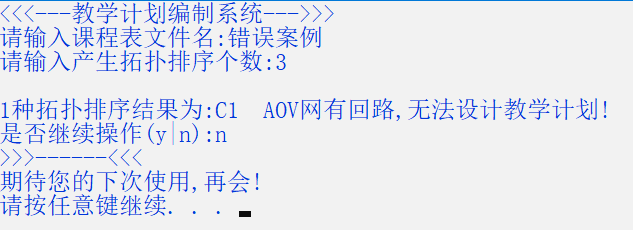
\includegraphics[width=300pt]{错误.png}
\caption{错误案例}
\end{figure}

\section{心得体会}
这次课程设计的心得体会通过实践我们的收获如下:\par
1.通过这次教学计划编制问题的课程设计,我们更深刻地了解了拓扑排序的特点与用法。\par
2.在实现拓扑排序时,一开始采用栈的数据结构,发现无法产生多种序列,于是选择利用线性表的特点实现。\par
3.最初读取文件时采用的方法是同时读取课程编号和先决条件,将每个顶点的入度打印出来观察发现C6的入度为0,于是找到了问题根源,从而解决了问题。

\newpage 
\section{附录}
\lstinputlisting[language=C]{main.c}

\end{document}
